\section{Analisi dello stato dell'arte}

La sicurezza delle informazioni viene definita utilizzando tre concetti di base:
confidenzialità, integrità e disponibilità, conosciuti anche con l'acronimo CIA (Confidentiality, Integrity e Avaiability).\\
%Per parlare di sicurezza delle informazioni al giorno d'oggi bisogna fare riferimento a tre concetti fondamentali: confidenzialità, integrità e disponibilità, conosciuti anche con l'acronimo CIA (Confidentiality, Integrity e Avaiability).\\
Per confidenzialità si intende la proprietà che impedisce a individui, entità o processi non autorizzati di accedere alle informazioni, per integrità si intende la proprietà dei dati che ne vieta l'alterazione accidentale o eseguita da una terza parte malevola, comprendendo il caso limite di generazione ex novo di dati, infine per disponibilità si intende la capacità di accedere in qualsiasi momento ai dati richiesti.\\
Il solo utilizzo di queste tre proprietà è stato spesso criticato perchè ritenuto troppo generale per essere effettivamente applicato durante l'ingegnerizzazione di sistemi.\\
Per questo motivo molti ricercatori e organizzazioni hanno cercato di estendere la CIA con altre proprietà, ad esempio con l'autenticazione utilizzata proprio nelle proprietà di confidenzialità e integrità.\\
L'estensione della CIA negli anni è documentata nell'articolo \cite*{SC14} ed è riassunta nella Tabella \ref*{tab:cia}.

\begin{table}[h!]
    \begin{tabular}{@{}lll@{}}
    \toprule
    \textbf{Anni} & \textbf{Definizione} & \textbf{Legenda}                                          \\ \midrule
    1970         & infosec = CIA        & Confidenzialità, Integrità, Disponibilità                 \\
    1980         & infosec += (Au,nR)   & Autenticazione e non-Ripudio                              \\
    1990         & infosec += CSpec     & Correttezza delle specifiche                              \\
    2000         & infosec += RITE      & Responsabilità, Integrità delle persone, fiducia, eticità \\ \bottomrule
    \end{tabular}
    \caption{Evoluzione della CIA}
    \label{tab:cia}
    \end{table}

%Da queste tre proprietà principali ne derivano altre utilizzate nella crittografia e implementate nei protocolli di sicurezza, tra queste troviamo la segretezza (o riservatezza) che impedisce all'avversario di ottenere alcune informazioni sui dati manipolati dal protocollo e l'autenticazione che identifica i partecipanti al protocollo, ad esempio se un partecipante A esegue il protocollo con il partecipante B, allora anche il partecipante B deve eseguire il protocollo con il partecipante A, inoltre si richiede ch eA e B condividano gli stessi valori dei parametri del protocollo.\\

\noindent Per raggiungere obiettivi di sicurezza, come confidenzialità o autenticazione dei dati nella rete, anche in presenza di attaccanti, si sono sviluppati i protocolli di sicurezza, questi ultimi descrivono come gli agenti si scambiano messaggi utilizzando le primitive crittografiche.\\
Gli errori di sicurezza non possono essere rilevati dal test funzionale del software perché appaiono solo in presenza di un attaccante, quindi l'utilizzo di tool automatici per la verifica può essere utile per ottenere reali garanzie sulla correttezza dei protocolli di sicurezza.\\ 
L'utilizzo dei protocolli di sicurezza nella maggior parte delle applicazioni sviluppate ha aperto un area di ricerca molto importante, infatti si cerca di progettare protocolli sempre più sicuri.\\
Sin dal 1983 con la ricerca di Dolev-Yao si è cercato un modo per dimostrare che un protocollo soddisfasse determinate proprietà di sicurezza, per fare questo sono nate due tecniche per testare la correttezza dei protocolli.\\
La prima tecnica è conosciuta come modello computazionale (o crittografico), mentre la seconda tecnica è conosciuta come modello simbolico (o metodo formale).\\
Queste due tecniche si basano sulla matematica formale per l'esecuzione di protocolli in ambienti con la presenza di uno o più attaccanti, l'obiettivo è quello di definire formalmente le proprietà di sicurezza previste dal sistema crittografico e sviluppare metodi per dimostrare rigorosamente la soddisfazione delle stesse.\\
Le caratteristiche principali del modello computazionale sono i modelli per l'esecuzione del sistema dettagliati a livello di bit e l'utilizzo di un attaccante potente, la sicurezza viene valutata rispetto a macchine probabilistiche a tempo polinomiale e questo fa si che in caso di esito positivo, le dimostrazioni di sicurezza forniscano delle garanzie.\\
In questo modello, la lunghezza delle chiavi è determinata da un valore chiamato security parameter, e la durata dell'esecuzione dell'avversario dovrebbe essere polinomiale rispetto al security parameter.\\
Tuttavia utilizzando questo modello anche su protocolli di piccole dimensioni le dimostrazioni di sicurezza sono molto lunghe, difficili e soggette ad errori.\\
Nel modello simbolico si utilizza una visione astratta dell'esecuzione del protocollo in quanto i messaggi scambiati dai partecipanti sono termini simbolici.\\
Inoltre si assume che le primitive di sicurezza siano delle black box assolutamente sicure (perfect cryptography), ad esempio l'attaccante non può ottenere il testo in chiaro da un testo cifrato senza essere a conoscenza della chiave corretta per la decifratura.\\
Questo fa si che la modellazione di un protocollo con il modello simbolico sia più semplice rispetto a quella con il modello computazionale e che anche le dimostrazioni di sicurezza siano più semplici, anche se l'alto livello di astrazione rende poco chiare le garanzie di sicurezza offerte.\\
A causa del diverso insieme di strumenti e tecniche, i due modelli hanno convissuto e si sono sviluppati in modo indipendente per molti anni.\\
Negli anni si è cercato di ridurre il gap tra i due modelli, i primi sono stati Abadi e Rogway \cite{AR00}, i quali hanno svolto ricerche sulla correttezza del modello computazionale chiedendosi sotto quali condizioni i messaggi simbolicamente equivalenti, intercettati da un attaccante passivo, sono anche equivalenti computazionalmente.\\
La loro ricerca ha portato ad ulteriori ricerche nell'ambito della correttezza del modello computazionale, riassunte nell'articolo di Cortier, Kremer, Warinschi\cite{CSW11}, nel quale gli autori ripercorrono le varie tappe della ricerca da quella di Abadi e Rogway allo sviluppo del tool CryptoVerif di Blanchet.\\
Nella Figura \ref*{fig:st} è possibile vedere come si è sviluppata la ricerca e quali sono le possibili strade future da intraprendere per nuovi studi.\\
Allo stato dell'arte si pensa che la verifica dei protocolli attraverso il modello simbolico abbia raggiunto un buon livello di maturità, anche se alcuni aspetti richiedono ulteriori ricerche.\\
Inoltre il modello simbolico si presta meglio ad essere automatizzato, a differenza del modello computazionale che fino a poco tempo fa richiedeva che le verifiche fossero fatte a mano (un esempio di tool automatico non ancora completo è il sopracitato CryptoVerif).\\ 
Per questo motivo da questo momento in poi verranno trattati solo tool per la verifica automatica di protocolli che utilizzano il modello simbolico.\\

\begin{figure}[h!] 
    \centering 
    \fbox{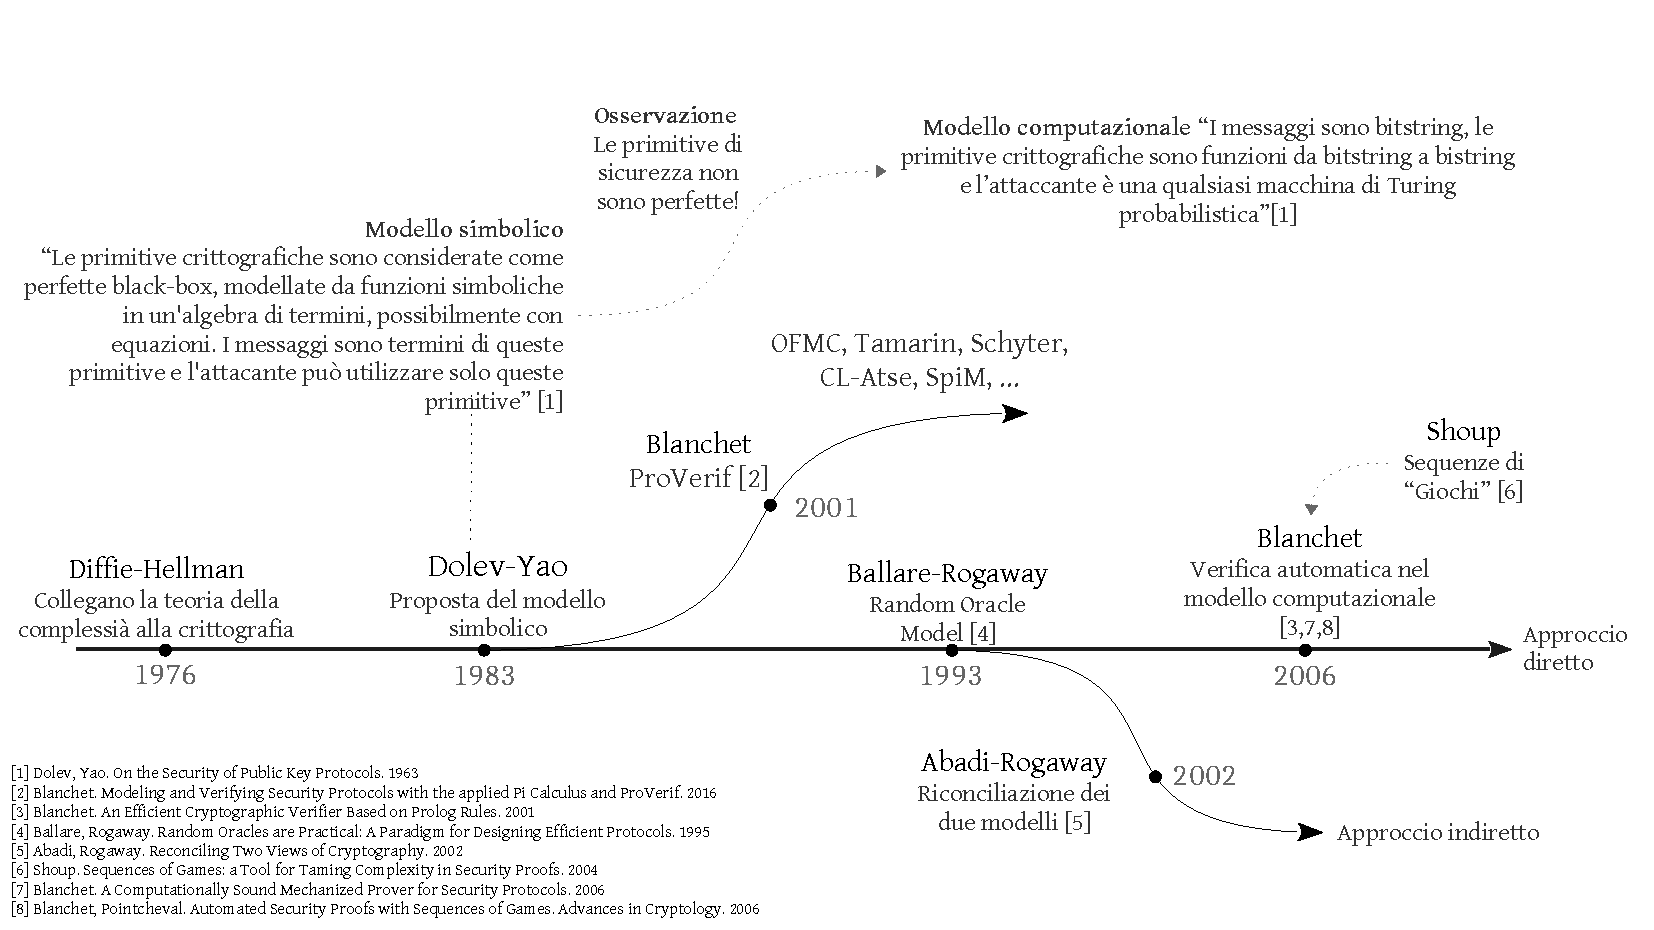
\includegraphics[width=\textwidth]{img/evolution.pdf}}
    \caption{Evoluzione della ricerca negli anni}
    \label{fig:st} 
\end{figure}
\newpage


